\chapter{Introduction}\label{chintro}
In today's software ecosystem, it has become imperative to give mathematical guarantees for the behaviour of a software with respect to its requirements. \Gls{Formalverification} is the procedure to ensure the correctness of a system with respect to a desired property by checking whether a mathematical model of the system satisfies a specification.
There are various \emph{formal} techniques to verify a software system. The applicability and usage of a formal technique depends on various factors such as, the type of software, the stage of the software development life cycle where verfication is performed, the resources available for verification. For instance, in the design stage, it maybe possible to verify properties on the abstraction of a system, such as model checking (cf. p8,~\cite{Baier2008PMC}). In the implementation stage, a more dynamic monitoring of the system behaviour and verification might be required such as runtime verification~\cite{bartocci2018}, where one works directly with the system (as opposed to an abstraction of it) and on select execution traces of the system (as opposed to all execution traces as in model checking), or depending on the resources, one might want to perform a check and provide correctness guarantees before deployment of the software such as static analysis~\cite{StaticAnalysis24}. The characteristics of the software system play a huge role in the selection of the formal technique that is adopted, such as if the interactions occur one after the other (sequential behaviour), if the interactions occur in parallel (concurrent behaviour), or if the interactions occur in parallel and can be made to occur one after the other (serializable), or if the system properties can be parameterized. We take the perspective of analyzing suitable ways to formally verify a particular software system.


In this work, we focus on unbounded client server systems where there is unbounded concurrency in the interaction between the clients and the servers as well as unboundedness in the number of clients (the number of clients is not known apriori). A first challenge is to identify the suitable representation of unbounded client server systems, we explore well known models in literature by varying their expressivity such as Petri nets, $\nu$-nets (Petri nets with names), and Elementary Object Systems (Petri nets with nesting). Another challenge is to identify the suitable way to specify the properties of the unbounded client server systems, we work with various temporal logics such as Linear Temporal Logic, Linear Temporal Logic with integer arithmetic, a variant of First Order Logic with monodic restriction. Now that the system can be represented using a suitable formal model and the property can be specified using an appropriate logic, the consequent challenge is to identify the formal technique by which to verify the system against its specifications. According to studies by NASA and the Systems Sciences Institute at IBM~\cite{ErrorCE10, SDLC10}, the error costs associated with identifying mismatches between requirements and the implemented software at a later stage of the software development lifecycle grow exponentially as the software goes through its development lifecycle. Therefore, we would like to use model checking to verify the unbounded client server systems at the design stage, in order to give formal guarantees early on, and avoid the high error cost. There are also other formal techniques in the design stage, such as equivalence checking, where one verifies whether two different mathematical models of a design represent the same behaviour. However, this is not interesting in our application.

\Gls{ModelChecking} is a formal  verification technique which allows for desired behavioral properties of a given system to be verified on the basis of a suitable model of the system through systematic inspection
of all states of the model. This is a technique that can be used in the design stage of the software development lifecycle. Model checking is a verification technique that has the following features. The  software (to be verified) is abstracted into a suitable mathematical \emph{model} and the various behaviours of the \emph{model} are identified as \emph{states}. Those \emph{states} that are possible from the initial setup of the model are called \emph{reachable states}. As stated earlier, the requirements to be verified are formulated using \emph{temporal logic}, it is temporal, to account for the time based properties. The reachable states of the system are traversed to verify the temporal logic properties. If the property fails, we obtain a sequence of states, known as the counterexample. Hence, it is automatic. Thus, model checking can be summarized as an algorithmic technique for checking temporal properties of systems. The model checking problem is also described as:
Given a system $P$ and a specification $\alpha$ on the runs of the system, decide whether system $P$ satisfies specification $\alpha$. This consists of checking that all runs of $P$ constitute models for $\alpha$. It suffices to show that no run of $P$ is a model for $\neg \alpha$, which is the same as checking that the intersection of the language accepted by $P$ and the language defined by $\neg \alpha$ is empty. For complex systems with millions of states, model checking can quickly run into the state space explosion problem~\cite{ClarkeKNZ11}. If there was a system with $n$ components and each component contained $m$ states, the composition of those components, would contain $m^n$ states, thereby exponentially incrementing the number of states.
Techniques~\cite{ClarkeStateSpace87,Clarke2012} to address this problem are described here. \Gls{SymbolicModelChecking} is a methodology where instead of explicitly checking all the states of the system, symbolic model checking algorithms manipulate sets of states~\cite{BiereTACAS99}.
Another approach is verifying representatives of the system or abstractions of the system wherein parts of the system are abstracted so that only the essential properties being verified are preserved in the abstraction~\cite{PeledAllForOneCAV93}.
In compositional verification, each component is verified separately and the overall correctness of the system is inferred~\cite{CompositionalVerificationNets98}.
While performing on-the-fly verification, instead of explicitly precomputing all the states, the state space is generated while the verification procedure is underway~\cite{Ontheflytpn09,Ontheflycpn21}.
There are also a set of partial order reduction techniques. For instance, in asynchronous systems where many events are independent of each other, they can be executed in arbitrary order without affecting the outcome of the computation and some redundancy can be avoided, thereby tackling the state space explosion~\cite{PartialOrderGodefroid96}. There is a notion of unfoldings in partial orders that reduces state space explosion~\cite{UnfoldingEsparza94}. In counter example guided abstraction refinement, while verifying properties,the counterexamples that are obtained are used to refine the initial abstraction~\cite{cegar03}.

Among these various techniques, we focus on model checking on \emph{bounded} (finite) runs of the system, and restricting the \emph{state space}. This technique is called \emph{bounded} model checking, which is illustrated in Fig.~\ref{figbmc}. In order to describe the behaviours of infinite state systems, such as unbounded client server systems, it is useful to think of automata that accept languages of infinite words, which we shall explore in the upcoming section.

\section{Infinite State Systems}
In this section, we explore automata that accept languages of infinite words such as \acrfull{BA}~\cite{Thomas90,Buchi1962DecisionMethod}. Later on, we shall describe \acrfull{PN}, which can directly represent behaviours of the infinite state systems with concurrency (See Sec.~\ref{sec:pn})\footnote{Alternatively, one might make a product automata to accept languages of infinite words where the underlying model allows for concurrency. However, Petri nets are a more elegant representation.}.
The term $\omega$- regular languages, describes the class of languages over infinite words, which is accepted by finite state machines. An infinite word ($\omega$-word) $\alpha \in \Sigma^{\omega}$, is an infinite sequence of symbols from the alphabet $\Sigma$. The infinite word can be represented as a function $\alpha : \mathbb{N}_{0} \rightarrow \Sigma$. In order to refer to the letter at the $i$th position, we use $\alpha(i)$.
For a finite sequence $[m\ldots n]$, $m,n \in \mathbb{N}_{0}, m\leq n$, we denote $\{m,\ldots,n\}$. Hence, $\alpha[m\ldots n]$ denotes the finite word occurring between positions $m$ and $n$,
$\alpha(m)\alpha(m+1)\ldots\alpha(n)$. It follows that $[m\ldots]$ denotes the infinite word $\alpha(m)\alpha(m+1)\ldots$ starting at $m$. Suppose $S$ is a set and $\sigma$ is an infinite sequence of symbols over $S$, $\sigma: \mathbb{N}_{0} \to S$. Then, $inf(\sigma)$ denotes the set of symbols in $S$ that occur infinitely often in $\sigma$. It can be formally defined as: $inf(\sigma)=\{s\in S | \exists^\omega n \in \mathbb{N}_{0}: \sigma(n)=s \}$.

\begin{dfn}
    An automaton is defined as a triple $A=(S,\to,S_{in})$ where $S$ is a finite set of states, $S_{in}\subseteq S$ is the set of initial states, and $\to \subseteq S \times \Sigma \times S$ is the transition relation. In case of deterministic automaton, $\to$ is a function from $S \times \Sigma \to S$.
\end{dfn}

\begin{dfn}\label{dfnbuchi}
    A \acrfull{BA} is denoted by $(A,G)$, containing an automata $A=(S,\to,S_{in})$
    and its \emph{good} states $G\in S$. We describe this with Example~\ref{RunExample}.
\end{dfn}

\begin{dfn}
    A run of a \gls{BA}, is a legal sequence of states that an automaton can pass through while reading the input $\alpha$.
    Let $A=(S,\to,S_{in})$ be an automaton and $\alpha: \mathbb{N}_0 \to \Sigma$  be an input word. A run of $A$ on $\alpha$ is an infinite sequence $\rho: \mathbb{N}_0 \to S$ such that $\rho(0) \in S_{in}$ and $\forall i \in \mathbb{N}_0,\rho(i)\xrightarrow{ \alpha(i)} \rho(i+1)$.
    A run of $A$ on the finite word $w = a_0a_1\ldots a_m$ is a sequence of states $s_0s_1\ldots s_{m+1}$ such that $s_0 \in S_{in}$ and $\forall i \in [0\ldots m], s_1\xrightarrow{\alpha(i)} s_{i+1}$.
\end{dfn}



\begin{eg}

    \begin{figure}[ht]
        \centering
        \begin{tikzpicture}[shorten >=1pt,node distance=2cm,on grid,auto]
            \node[state,initial] (q_0)   {$q_0$};
            \node[state,accepting] (q_1) [above right=of q_0] {$q_1$};
            \node[state] (q_4) [right=of q_1] {$q_4$};
            \node[state] (q_2) [below right=of q_0] {$q_2$};
            \node[state,accepting](q_3) [right=of q_2] {$q_3$};
            \path[->]
            (q_0) edge  node {a} (q_1)
            edge  node [swap] {a} (q_2)
            edge [loop above] node {a,b} ()
            (q_1) edge [loop above] node {a} ()
            edge  node  {b} (q_4)
            (q_2)  edge  node [swap] {a} (q_3)
            (q_3)  edge node {b} (q_4)
            edge[above, bend left=10] node {b} (q_2)
            (q_4)   edge [loop above] node {a,b} ();
\end{tikzpicture}
        \caption{A \gls{BA} accepting the $\omega$-word $\alpha=abbaabababa\ldots$}
        \label{RunExample}
    \end{figure}

    Consider the above figure with $F=\{q_1,q_3\}$ and the $\omega$-word $\alpha=abbaabababa\ldots$, some of the possible runs on $\alpha$ are given below:

    \begin{figure}[!ht]
        \centering
        \begin{tabular}{llllllllllllllllllllll}
              & a &       & b &       & b &       & a &       & a &       & b &       & a &       & b &       & a &       & b$\ldots$               \\


        $q_0$ &   & $q_0$ &   & $q_0$ &   & $q_0$ &   & $q_0$ &   & $q_0$ &   & $q_0$ &   & $q_2$ &   & $q_3$ &   & $q_2$ &           & $q_3\ldots$ \\

        $q_0$ &   & $q_0$ &   & $q_0$ &   & $q_0$ &   & $q_1$ &   & $q_1$ &   & $q_4$ &   & $q_4$ &   & $q_4$ &   & $q_4$ &           & $q_4\ldots$ \\

        $q_0$ &   & $q_0$ &   & $q_0$ &   & $q_0$ &   & $q_0$ &   & $q_2$ &   & $q_3$ &   & $q_2$ &   & $q_3$ &   & $q_2$ &           & $q_3\ldots$
\end{tabular}
    \end{figure}

\end{eg}

\subsubsection{Acceptance Condition}
B{\"u}chi automaton accepts an input if there is a run along which some subset of $G$ occurs infinitely often~\cite{Kupferman2018}. Since $G$ is a finite set, it is easy to see that there must actually be a state $g \in G$ that occurs infinitely often along $\sigma$. In other words, if we regard the state space of a B{\"u}chi automaton as a graph, an accepting run traces an infinite path that starts at some state $s \in S_{in}$, reaches a good state $g \in G$ and loops back to $g$ infinitely often. In the infinite accepting run shown in Fig.~\ref{Accepting run}, the move from state $s$ to state $g$ is the non-looping part, that we call \emph{stem}, which ends in the \emph{loop} at state $g$.

\begin{figure}[ht]
    \centering
    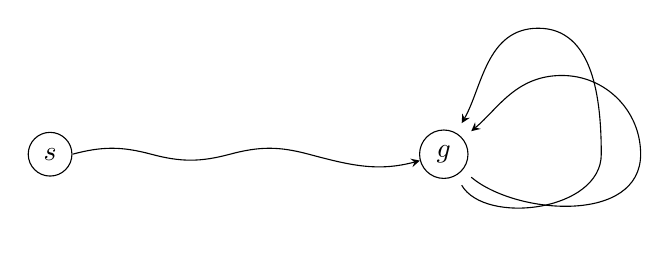
\begin{tikzpicture}
\path node[circle,draw] (s) {$s$} ++ (5,0) node[circle,draw] (g) {$g$};
\draw[-stealth] (s.east) to[out=15,in=165] ++ (1,0)
        to[out=-15,in=-165] ++ (1,0) to[out=15,in=165] ++ (1,0)
        to[out=-15,in=-165](g);
\draw[-stealth,shorten >=4pt,shorten <=4pt] (g) to[out=-40,in=-90] ++ (2.5,0) to[out=90,in=0]
        ++ (-1,1) to[out=180,in=40] (g);
\draw[-stealth,shorten >=4pt,shorten <=4pt] (g) to[out=-60,in=-90] ++ (2,0) to[out=90,in=0]
        ++ (-0.8,1.6) to[out=180,in=60] (g);
\end{tikzpicture}
    \caption{Accepting run of a \gls{BA}}
    \label{Accepting run}
\end{figure}

\begin{figure}[!ht]
    \centering
    \scalebox{0.7}{\input{figures/fig_bmc}}
    \caption{Bounded Model Checking}
    \label{figbmc}
\end{figure}

\begin{eg}
    We illustrate bounded model checking in Figure.~\ref{RunExample}, where we would like to check the temporal property that the letter $a$ occurs sometime in the future and reoccurs infinitely often. Now, this can occur, in a non-looping \emph{stem} part of the run, or in the infinite \emph{loop} of the run (cf.Fig.~\ref{Accepting run}). Notice that the initial state $q_0$ does not accept the letter \emph{a}. In order to know, if there is some state, where \emph{a} is accepted in the future, one needs to look at the next states, apart from the initial state. Using the principle of bounded model checking, we check if \emph{$\neg$ a} is accepted in a \emph{stem} or in \emph{loop} of all the runs possible in the model. The presence of an accepting run, acts as a counterexample to the property being checked. In this case, the sequence of states $q_0,q_2,q_3,q_2,q_3,\ldots$ is a counterexample trace. We can also view this as reaching a state, that accepts the said property.
\end{eg}

In  Chapter.~\ref{chlogics}, we describe how to formally specify the properties in a formal manner using a logical language.
One drawback is that we cannot explicitly represent concurrency in this model, hence we look at more suitable models to represent concurrency in unbounded client server systems via Petri nets, $\nu$-nets (Petri nets with names), and Elementary Object Systems (Petri nets with nesting) in Chapter.~\ref{chmodels}. We revisit this notion of automatically performing bounded model checking, while verifying various models and properties in Sec.~\ref{sec:encodingLTL} and Sec.~\ref{ssec:verif} using a set of specialized tools called SAT/SMT solvers. Given a set of constraints, such as in bounded model checking, SAT/SMT solvers can efficiently check if there exists a \emph{satisfying assignment} of values to those constraints. SAT solvers work with Boolean values. SMT solvers offer various underlying theories such as bit vectors and integer arithmetic~\cite{MouraB08,BarbosaBBKLMMMN22}.



\section{Contributions}
In this thesis, we focus on verification of unbounded client server systems and representing them by various suitable formal models as well as verifying the properties of the systems specified using various logics. In this system, there are unbounded interactions between the single server and unboundedly many clients that are not known apriori. The interactions are restricted to requests by the clients that are responded to, by the server. We have not worked with systems where there are interactions between the clients, nor have we worked with the multiple server multiple client systems. These extensions can be interesting future work.
The major contributions of this work are the following:

\begin{enumerate}

    \item \textbf{Formulated the $2$D-BMC algorithm}. We extend the standard \acrfull{BMC} algorithm to two dimensional bounded model checking, i.e., $2$D-BMC that exploits the two dimensional unboundedness in the Petri nets representing the unbounded client server systems, i.e., unboundedness in the number of clients as well as unbounded concurrency. This is particularly helpful for verifying systems with true concurrency. (See Chapter.~\ref{chproblem})
    \item  \textbf{Verification of a Linear Temporal Logic with integer arithmetic properties on Petri nets using $2$D-BMC:} Built a tool to verify Linear Temporal Logic with integer arithmetic properties on Petri nets. The tool employs SMT solvers to perform the verification queries using an extension of BMC, called the $2$D-BMC algorithm. This tool competes with state of the art \Gls{PetriNet} verification tools and is the first of its kind to use various semantics of Petri nets. (See Chapter.~\ref{chltl})
    \item \textbf{Verification of a variant of  First Order Logic on Petri nets using $2$D-BMC:} Implemented a tool to verify properties of First Order Logic with monodic restriction on Petri nets with identifiers, called $\nu$-nets and which employs SMT solvers to perform the verification queries using $2$D-BMC algorithm. (See Chapter.~\ref{chmfotl})
    \item \textbf{Charted the decidability status of Elementary Object Systems:} The notion of coverability is to ask, given a model and its configuration, is there a second reachable configuration that is smaller than the original configuration. These are important questions in Petri nets and also by extension, in Elementary Object Systems (EOS), which are essentially nets with nesting. In the interactions in the EOSs, imperfect steps are possible, which we call lossiness. Lossiness can occur at various levels of nesting in the EOSs. We charted the decidability status of reachability and coverability problems in EOSs in the case of lossiness at various nesting levels. (See Sec.~\ref{sec:fullLossydecidability})
    \item \textbf{Verification of  reachability of Elementary Object Systems:} The notion of reachability is to ask if a particular configuration can be reached. We implemented an open source tool to verify reachability properties on a class of higher order Petri nets with nesting, called Elementary Object Systems. (See Sec.~\ref{sec:EOSTool})

\end{enumerate}





\begin{comment}

%\subsection*{$\omega$-regular expression}
\begin{dfn}
    An $\omega$-regular expressions is of the form $r_1 s_1^{\omega} +\ldots + r_n s_n^{\omega}$ with standard regular expressions $r_1 , s_1 ,\ldots , r_n ,s_n$.    The semantics of those expressions is defined in a manner analogous to standard regular expressions. For an expression $s$, which defines the language $U \subseteq \Sigma^*$ , the expression $s^\omega$ defines the $\omega$-language $U^\omega$.
\end{dfn}


\begin{eg}
    Consider the following $\omega$-regular expression~\cite{Mukund12}:
    \beq
    (a+b)^*a^\omega + (a+b)^*(ab)^\omega
    \enq

    The corresponding B\"uchi automaton can be drawn as follows:
    \begin{figure}[ht]
        \centering
        \input{figures/1_omegareg}
        \label{regular expression}
        \caption{$\omega$-regular expression}
    \end{figure}

\end{eg}
It may be useful to think in terms of $\omega$-regular expressions, as they can be helpful in characterising the B\"uchi automaton.

\subsubsection{Deterministic and Non deterministic Automata}

\begin{figure}[ht]
    \centering
     \begin{tikzpicture}[shorten >=1pt,node distance=2cm,on grid,auto]
\node[state,initial,accepting] (q_0)   {$s1$};
\node[state] (q_1) [ right=of q_0] {$s2$};
\path[->]
(q_0) edge[above, bend left=15]  node {b} (q_1)
edge [loop above] node {a} ()
(q_1) edge[loop above]  node {b} ()
edge[above, bend left =15] node{a} (q_0)
;
\end{tikzpicture}
    \caption{Deterministic automaton recognizing $L$}
    \label{DeterministicBA}
\end{figure}

Consider the language $L$ over $\{a, b\}$  containing all words that contain infinitely many occurrences of $a$. The deterministic automaton with two states recognizes $L$ with a  B\"uchi condition $\{s1\}$ as in Figure~\ref{DeterministicBA}.

Consider the complement of language $L$ over $\{a, b\}$, $\overline{L}$ set of all infinite words $\alpha$ such that $\alpha$ has only finitely many occurrences of $a$.
The automaton guesses a point in the input beyond which it will see no more $a$'s. There is no deterministic automaton recognizing $\overline{L}$. The automaton in Figure~\ref{NBA} accepts $\overline{L}$.

\begin{figure}[ht]
    \centering
    \begin{tikzpicture}[shorten >=1pt,node distance=2cm,on grid,auto]
\node[state,initial] (q_0)   {$s1$};
\node[state,accepting] (q_1) [ right=of q_0] {$s2$};
\path[->]
(q_0) edge[above]  node {b} (q_1)
        edge [loop above] node {a,b} ()
        (q_1) edge[loop above]  node {b} ();
\end{tikzpicture}
    \caption{Non deterministic automaton recognizing $\overline{L}$}
    \label{NBA}
\end{figure}
\end{comment}
